\documentclass[twoside,10pt]{article}
\usepackage{/Users/bradenhoagland/latex/styles/toggles}
%\toggletrue{sectionbreaks}
%\toggletrue{sectionheaders}
\newcommand{\docTitle}{Math 412 - HW 8}
\usepackage{/Users/bradenhoagland/latex/styles/common}
\importStyles{modern}{rainbow}{boxy}

%\renewcommand{\theenumi}{\alph{enumi}}

\begin{document}
%\tableofcontents

%--------------------------------------------------------------------------------
% problem 1
%--------------------------------------------------------------------------------
\begin{exer}[Lesson 16, 5 points]
        Let $f: \R^5 \to \R$ be the function defined in Lesson 16. Find $\nabla f(1, 2, 3, 4, 5)$ and $\nabla f(5, 1, 3, 4, 2)$. In other words, find $\dfrac{\partial f}{\partial x_i}$ for $i = 1, \dots, 5$.
\end{exer}

\textbf{First one:} The diagram at $(1,2,3,4,5)$ is below.

\begin{figure}[H]
	\centering
	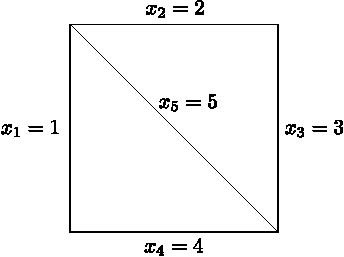
\includegraphics[scale=1]{fig/1a.pdf}
	%\caption{}
\end{figure}

Its 1-dimensional persistence diagram is $I_{[4,\infty)}\oplus I_{[5,\infty)}$. Thus the output of the function is $f(1,2,3,4,5) =  b_1^2 + b_2^2 = 4^2 + 5^2 = 41$. Note that $b_1=x_4$ and $b_2=x_5$, so the only $x_i$ affecting the output of $f$ at $(1,2,3,4,5)$ are $x_4$ and $x_5$. Thus the partial derivatives are
\[
\frac{\p f}{\p x_i} =
\begin{cases}
	2 b_1 = 8 & \text{if } i=4,\\
	2 b_2 = 10 & \text{if } i=5,\\
	0 & \text{else}.
\end{cases}
\] 
We can write this in gradient form as $\nabla_{}f(1,2,3,4,5) = (0,0,0,8,10)$.

\textbf{Second one:} The diagram at $(5,1,3,4,2)$ is below.

\begin{figure}[H]
	\centering
	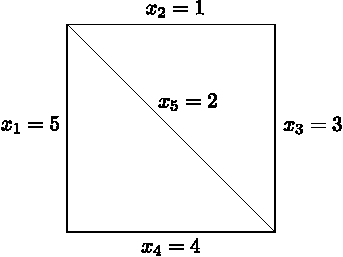
\includegraphics[scale=1]{fig/1b.pdf}
	%\caption{}
\end{figure}

The 1-dimensional persistence diagram is $I_{[3,\infty)}\oplus I_{[5,\infty)}$ this time, with $b_1 = x_3 = 3$ and $b_2 = x_1 = 5$. By a similar argument, the partial derivatives at this point are
\[
\frac{\p f}{\p x_i} =
\begin{cases}
	2b_1 = 6 & \text{if } i=3,\\
	2b_2 = 10 & \text{if } i=1,\\
	0 & \text{else}.
\end{cases}
\] 
We can write this in gradient form as $\nabla_{}f(5,1,3,4,2) = (10, 0, 6, 0, 0)$.

\end{document}
